\begin{figure*}[t]
    \centering
    \begin{subfigure}[b]{0.222\textwidth}
        \center
        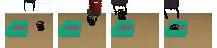
\includegraphics[width=3cm]{val/imgs/comparison_data/filmstrip_tray.jpeg}
        
        \vspace{0.1cm}
        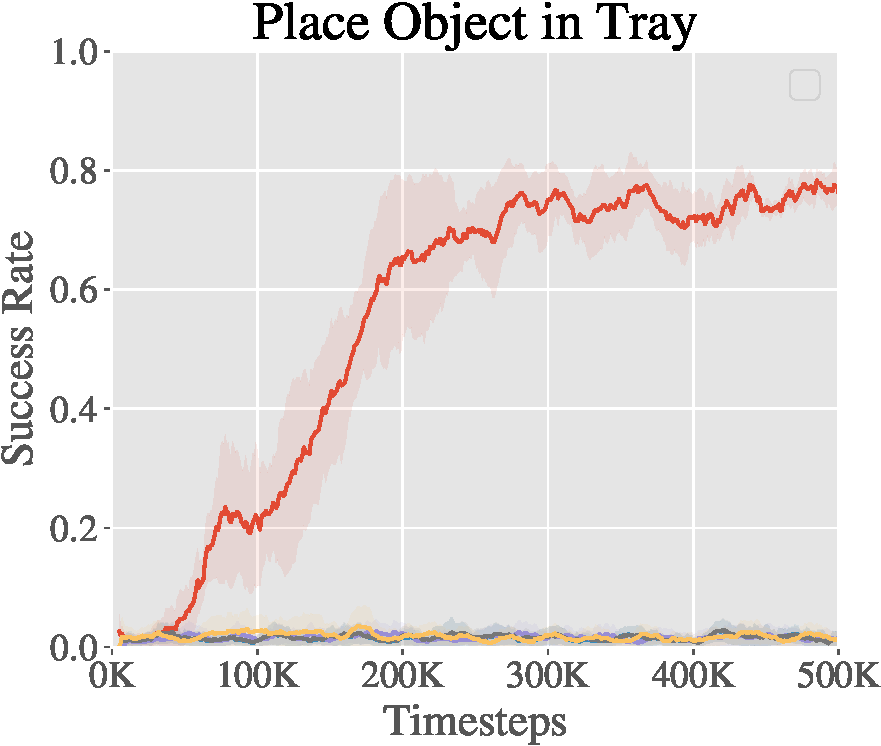
\includegraphics[width=0.95\textwidth]{val/imgs/comparison_data_new/plt4-crop.pdf}
    \end{subfigure}
    \begin{subfigure}[b]{0.21\textwidth}
        \center
        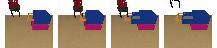
\includegraphics[width=3cm]{val/imgs/comparison_data/filmstrip_top.jpeg}
        
        \vspace{0.1cm}
        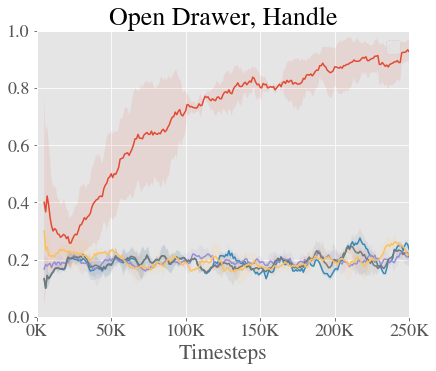
\includegraphics[width=1\textwidth]{val/imgs/comparison_data_new/fixed_handle.png}

    \end{subfigure}
    \begin{subfigure}[b]{0.21\textwidth}
        \center
        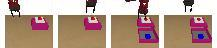
\includegraphics[width=3cm]{val/imgs/comparison_data/filmstrip_bottom.jpeg}
        
        \vspace{0.1cm}
        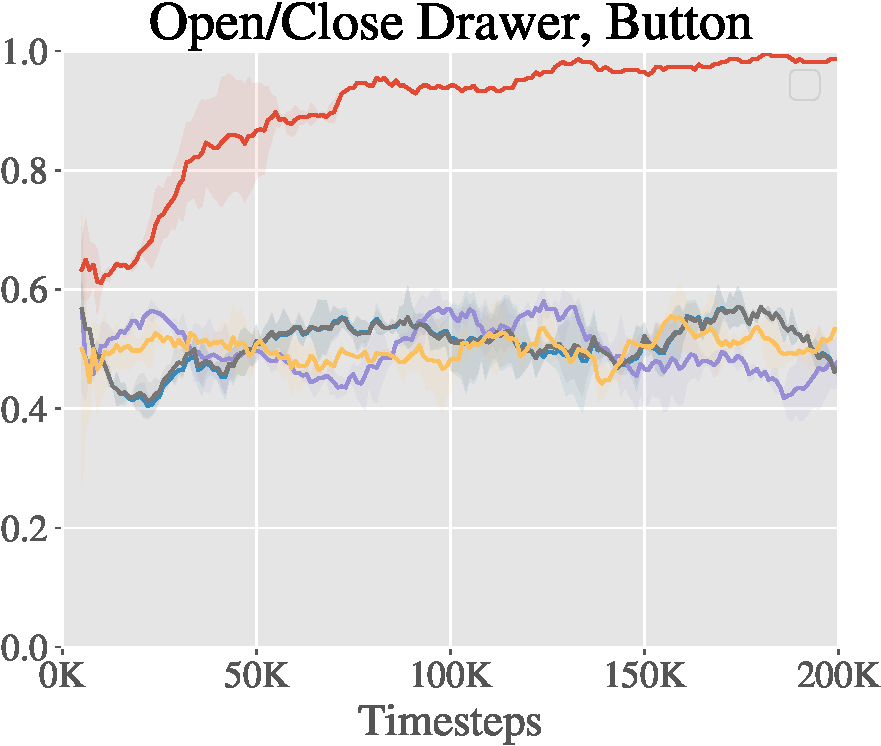
\includegraphics[width=1\textwidth]{val/imgs/comparison_data_new/plt2-crop.pdf}
    \end{subfigure}
    \begin{subfigure}[b]{0.21\textwidth}
        \center
        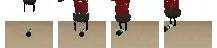
\includegraphics[width=3cm]{val/imgs/comparison_data/filmstrip_b.jpeg}
        
        \vspace{0.1cm}
        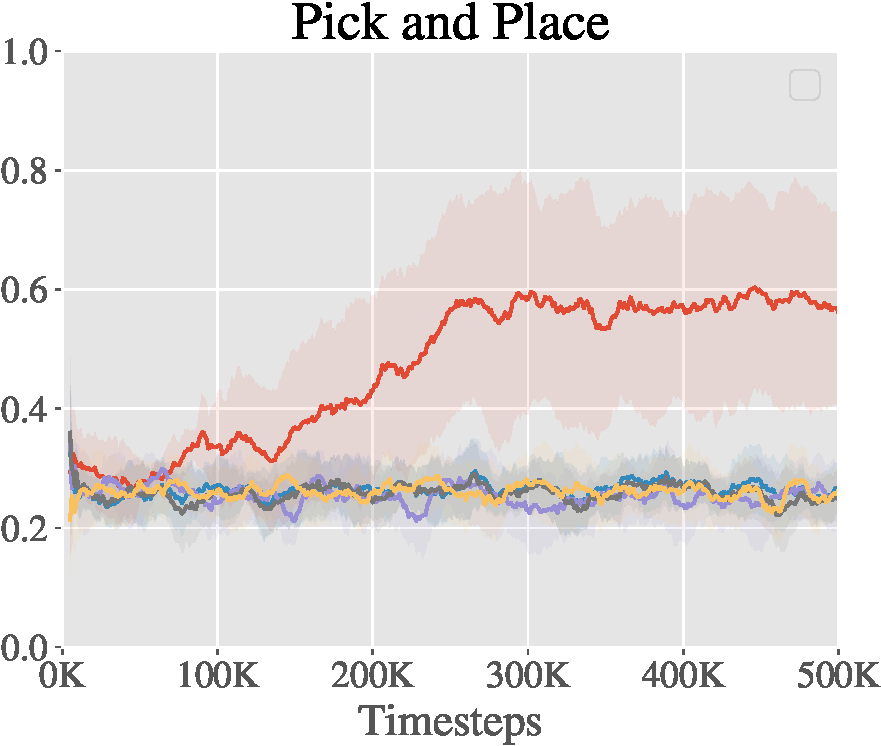
\includegraphics[width=1\textwidth]{val/imgs/comparison_data_new/plt3-crop.pdf}
    \end{subfigure}
    \begin{subfigure}[b]{0.1\textwidth}
        \center
        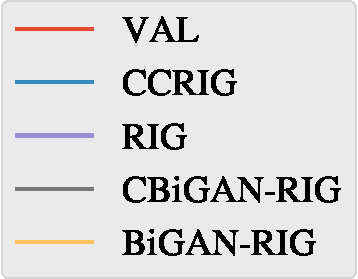
\includegraphics[width=1\textwidth]{val/imgs/comparison_data_new/legend-crop.pdf}
        \vspace{0.6cm}
    \end{subfigure}
    
    \caption{Learning curves for simulation experiments, fine-tuning on an unseen environment. Our method is able to learn these tasks online, while none of the baselines or prior methods are able to make meaningful learning progress in this setting. A successful rollout of each task in a test environment is shown above the corresponding plots. }
    \label{fig:sim_comparison}
    %\vspace{-0.5cm}
\end{figure*}